%
%=======================================
%  template.tex
%=======================================
%
\documentclass[12pt,titlepage,fleqn]{article}
\usepackage{amsmath}
\usepackage{amssymb}
\usepackage{latexsym}
\usepackage[round]{natbib}
\usepackage{xspace}
%\usepackage{epsfig}
\usepackage{graphicx}
\usepackage{bm}

% SPACING COMMANDS (Latex Companion, p. 52)
\usepackage{setspace}
\renewcommand{\baselinestretch}{1.0}
\textwidth 470pt
\textheight 690pt
\oddsidemargin 0pt
\evensidemargin 0pt

% see Latex Companion, p. 85
%\voffset     -50pt
\topmargin     0pt
\headsep      20pt
\headheight   15pt
\headheight    0pt
\footskip     30pt
\hoffset       0pt

% nicer fonts
\usepackage{times}

% self-defined commands
\include{newcommands}

% bibliography
\bibliographystyle{gji}

%======================================================
\begin{document}
%======================================================
\begin{spacing}{1.0} % empty lines are required!
\begin{center}

\Large {\vspace{0.1in} \bf \verb=GRID3D_FLEXWIN= Readme}
\end{center}

\end{spacing}

\verb=GRID3D_FLEXWIN= is re-written from my old \verb=GRID3D= program to adapt to the output of Alessia's \verb=FLEXWIN= package, and provide an unbiased initial solution for the \verb=cmt3d_FLEXWIN= program, although this best solution is only for a fixed depth. Notice the pre-processing step to pick the usable data and synthetic windows is exactly the same as stated in section 1 of the \verb=cmt3d_FLEXWIN= Readme file.
%=====%======================================================

\section{Parameter file}

For the structure of the program and subroutine calls, refer to \verb=call-graph=. The name of the parameter file is hard-wired in the main program: \verb=GRID3D.PAR=.

\begin{verbatim}
CMTSOLUTION
1.0e22                         -- dmoment
flexwin_T006_T030.output
.false.                        -- weigh_data_files
2 2 1  0  1.15 0.55 0.78       -- weights of data comp,az,dist
.false.                        -- station_correction
.true. 3                       -- global_search, ncalc
10 16 0.5                      -- strike
20 26 0.5                      -- dip
30 36 0.5                      -- rake
4.2 4.4 0.1                    -- Mw, only valid with local search
.true.                         -- write cmt-file-new
\end{verbatim}

The first line gives a cmt solution file name. Unlike \verb=cmt3d_flexwin=, this is only used to obtain a reasonable starting $M_w$ for global grid search, therefore may be elliminated in the future. However, since we are not short of initial solutions, I decided to keep it there. The data weighting procedures are exactly the same as outlined in the readme file for \verb=cmt3d_flexwin=. Station correction must be allowed for actual data (as oppose to synthetic data), which otherwise defeats the purpose of this program, although significantly longer search time should be expected with this extra operation.

Global search goes through \verb-strike=0:10:180-, \verb-dip=0:10:90-, \verb?rake=-180:30:180?, \verb-Mw=0.9:0.05:1.1*mw- in search for an optimal misfit value. Therefore the values listed in the next 4 lines are only used when \verb-global_search=.false.-, and ignored when \\
\verb-global_search=.true.-. Also \verb-ncalc- is only significant in the case of global search, where iteratively refined searches are done to pinpoint the global minimum.



\begin{itemize}
\item The output \verb=CMTSOLUTION_NEW= file can be copied directly to \verb=cmt3d_flexwin= as an initial cmt solution, and the corresponding synthetics should be calculated by the program \verb=xadd_frechet_derivatives=.
\item No synthetics is needed (derivative synthetics of course have to be present), since all the synthetic header information is taken from \verb=syn.Mrr= files.
\item New cmt solution will bear the name \verb-CMTSOLUTION_NEW-, which is hard-wired.
\item A typical search array size can be 20x20x40x5 for strike,dip,rake and Mw. although it is their product (80000) that really restricts the number of double-couple moment tensor sources that can be searched.
\end{itemize}

%============================================

\section{Plotting}

Although the program will output the best strike,dip,rake,Mw that ive rises to the global or local minimum of the misfit function, it is much more straightforward to read that information off some graphs. These graphs can also display visually the trade-off between different parameters, therefore, are more useful in terms of understanding the significance of our minimum solution.

The output files from the \verb-grid3d_flexwin- package have the names
\begin{verbatim}
 grid3d_misfit[.icalc].n_mw
\end{verbatim}
Each file documents the strike,dip,rake and corresponding minimum value (normalized by minimums for all Mw) for a particular choice of $M_w$, as well as a particular iteration of global search. I have written an auxilliary program to help produce plots to visualize this 3D function:
\begin{verbatim}
 plot_grid.pl grid-output-files
\end{verbatim}
For each output file, 6 strike, dip and rake are selected close to the global minimum, and corresponding slices are taken from the grid file. Each slice is plotted and contoured to show how the misfit varies as a function of two variables with other variables fixed. This script is by no means general, since it is very hard to write general GMT programs that will fit all cases. But the users can play around either with this perl script or the ouput bash file for fine tuning. The perl script used some perl libary files that are available for Caltech/GPS users. A sample output is attached to this readme.

\begin{figure}
\begin{center}
     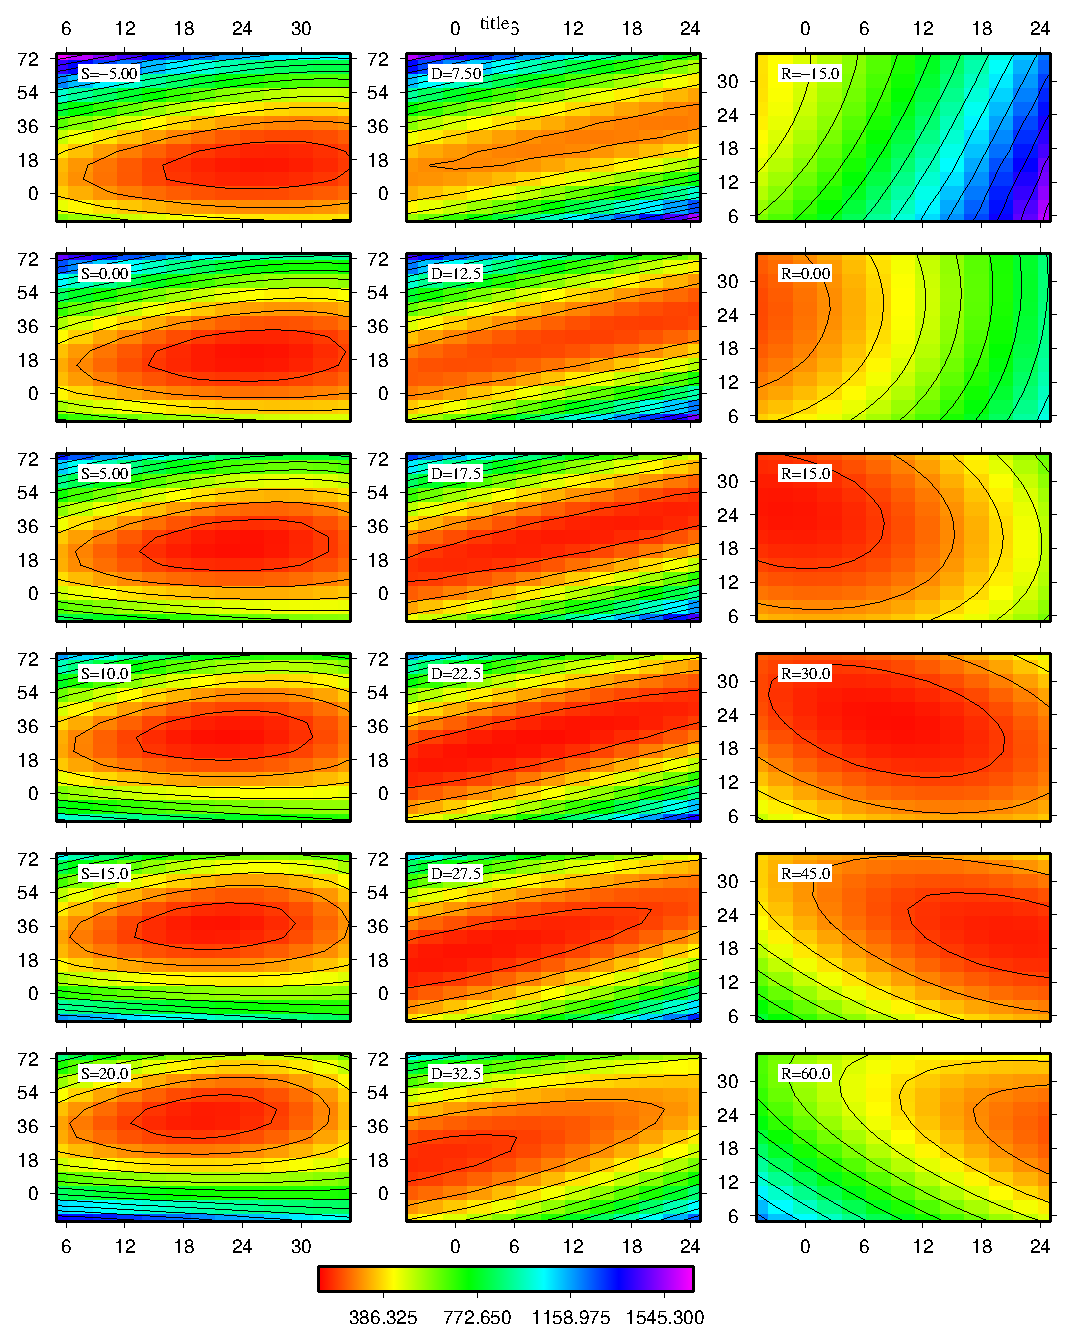
\includegraphics[width=6in]{grid_0.eps}%
  \end{center}
\end{figure}

%=======================================================

\end{document}
